\section{АНАЛИТИЧЕСКИЙ ОБЗОР ПРОГРАММНЫХ ПРОДУКТОВ, ЛИТЕРАТУРНЫХ ИСТОЧНИКОВ}

\subsection{Общие понятия о навигации мобильных систем}

Навигация мобильных систем представляет собой процесс определения положения
устройства в пространстве и его перемещения в соответствии с заранее заданными
целями. Эта область охватывает множество технологий и методов, включая системы
позиционирования, карты и алгоритмы планирования маршрутов. Мобильные системы
могут быть использованы в самых разных сферах — от автономных транспортных
средств до мобильных роботов в промышленных и исследовательских приложениях.

Для навигации используются различные сенсоры для сбора информации о
своем окружении. Это могут быть камеры, лазерные дальномеры, ультразвуковые
датчики, IMU. Собранные данные обрабатываются с помощью
специализированных алгоритмов, что позволяет системе точно определять свое
положение и вносить изменения в маршрут в реальном времени. Успешная навигация
зависит от способности системы адаптироваться к изменениям в окружающей среде,
таким как перемещения других объектов, препятствия или изменения в маршруте.

\subsection{SLAM}

Для одновременной локализации и построения карты в мобильной навигации является
SLAM (Simultaneous Localization and Mapping — одновременное определение
положения и построение карты). Эта технология позволяет одновременно строить
карту окружающего пространства и определять свое местоположение относительно
этой карты, не имея предварительной информации о среде.

SLAM представляет собой не только способ построения карты, но и инструмент для
локализации — определения текущего положения системы в уже созданной карте. Это
особенно важно для мобильных роботов и автомобилей, которые не могут оперировать
в заранее определенных пространствах и нуждаются в создании карты окружающей
среды в процессе своего движения. Основная задача SLAM — это совместное решение
проблемы локализации и картографирования.

% Формальная постановка 

Задача SLAM заключается в вычислении оценки метоположения $x_t$ агента и карты
окрущающей среды $m_t$ из ряда наблюдений $o_t$ над дискретным временем с шагом
дискретизации $t$. Все перечисленные величины являются вероятностными. Цель
задачи состоит в том, чтобы вычислить $P(m_t, x_t | o_{1:t})$. Применение правила
Байеса является основой для последовательного обновления апостериорного
местоположения, учитывая карту и функции перехода~$P(x_t, x_{t-1})$:

\begin{equation}
P(x_t | o_{1:t}, m_t) = \sum_{m_{t-1}} P(o_t | x_t, m_t) \sum_{x_{t-1}} P(x_t |
	x_{t-1}) P(x_{t-1} | m_t, o_{1:t-1})
\end{equation}

Точно так же карта может обновляться последовательно:
\begin{equation}
P(m_t | x_t, o_{1:t}) = \sum_{x_t} \sum_{m_t} P(m_t | x_t, m_{t-1}, o_t)
	P(m_{t-1}, x_t | o_{1:t-1}, m_{t-1})
\end{equation}

Процесс SLAM можно разделить на несколько ключевых этапов. Сначала система
начинает с неопределенности относительно своей позиции и окружающей среды. С
помощью сенсоров она собирает данные о ближайших объектах, которые используются
для построения карты. На основе этой информации система оценивает, где она
находится, и корректирует свои вычисления с учетом новых данных. Постоянное
обновление карты и позиции позволяет системе поддерживать точность навигации,
несмотря на ошибки и неопределенности.

Помимо построения карты, мобильные системы навигации должны также учитывать
задачу нахождения маршрута между двумя точками на карте. Задача построения
маршрута должны учитывать габариты робота для создания маршрутов которые
возможно выполнить, а также высчитывать оптимальный маршрут на основе
пройденного расстояния и дистанции от ближайших препятствий.

Важной составляющей навигации является исполнение маршрута. Как только
оптимальный путь найден, система должна эффективно следовать этому маршруту,
корректируя свое движение при необходимости. Для этого используется целый набор
методов, включая управление движением, обработку сенсорных данных и системы
коррекции ошибок, избеганием препятствий. В процессе исполнения маршрута система
может столкнуться с различными непредсказуемыми ситуациями, такими как внезапное
появление препятствий или необходимость обхода объектов, что требует гибкости в
принятии решений.

Одной из главных сложностей в SLAM и навигации мобильных систем является работа
в динамических и изменяющихся условиях. Окружающая среда может быть не только
сложной и многообразной, но и динамичной — например, в случае движения других
объектов, изменения освещенности или появления новых препятствий. В таких
условиях мобильные системы должны постоянно обновлять свои карты и маршруты,
чтобы оставаться эффективными и безопасными. Это требует не только точных
сенсоров, но и быстрых алгоритмов обработки данных.

\subsection{Анализ существующих программных решений по теме дипломного
проектирования}

Программные фреймворки играют ключевую роль в разработке программного
обеспечения, предоставляя инфраструктуру для создания, тестирования и внедрения,
решая типовые задачи и позволяют сфокусироваться на разработке функционала
продукта. Однако, в области автономной навигации роботизированных платформ
многие разработки остаются закрытыми, что связано со спецификой определённых
проектов и их проприетарным характером. Несмотря на это, в индустрии широко
используется программное обеспечение с открытым исходным кодом.

В программировании роботов активно используются фреймворки для межпроцесного
взаимодействия между отдельными модулями\footnote{Под модулями подразумеваются
отдельные программы, являющиеся компонентами системы, исполняющиеся в отдельных
процессах операционной системы, или даже на отдельных компьютерах.}. Примером
таких фреймворков служат \ros{} и YARP.
h
Это позволяет разрабатывать ПО с использованием разных языков программирования,
осуществлять переиспользование отдельных модулей, анализировать и записывать
потоки сообщений, настраивать маршрутизацию сообщений.

\ros{} является де-факто стандартным фреймворком для программного обеспечения
роботизированных систем \cite{albonico2023software}. Основополагающая статья

\selectlanguage{english}
"Software engineering research on the Robot Operating System: A systematic
mapping study"
\selectlanguage{russian}
\cite{quigley2009ros} процитирована более
\num{13000} раз.

Yet Another Robot Platform (YARP) \cite{metta2006yarp} -- это фреймворк который
преследует цели, очень схожие с \ros{}. YARP поддерживает построение системы
управления роботом как набор программ общающимся в одноранговой сети используя
различные каналы связи, что по своей сути не отличается от целей ros{}. YARP
менее популярен и используется для более специализированных систем и не имеет
отличительных преимуществ, поэтому далее его не рассматриваем.

\ros{} это распределённый фреймворк из процессов (также известных как
\textit{ноды}), который позволяет разрабатывать исполняемые файлы индивидуально,
и свободно сочетать их во время исполнения. Эти процессы могут быть объединены в
\textit{пакеты} и \textit{стэки}, которыми можно легко делится и распространять.
\ros{} поддерживает единую систему кодовых \textit{репозиторириев} которые
позволяют сотрудничеству быть распределённым.

Философские цели \ros{} можно кратко сформулировать следующим образом
 \cite{quigley2009ros}:
\begin{itemize}
	\item P2P;
	\item Основанный на инструментах;
	\item Многоязычный;
	\item Тонкий;
	\item Свободный и открытый исходный код.
\end{itemize}

На данный момент существует две версии \ros{}: \ros{} 1 и \rosTwo{}. Первый
официальный релиз \ros{} (под кодовым названием ROS Box Turtler) состоялся 2
марта 2010 года. Первый официальный релиз \rosTwo{} состоялся 8 декабря 2017
года. \rosTwo{} это более расширенная версия \ros{}, спроектированная чтобы
устранить недостатки \ros{} 1, такие как: масштабируемость, производительность и
кросс-платформенная совместимость, используя Data Distribution Service (DDS) для
общения и вводя новые понятия, такие как жизненный цикл ноды и качество
обслуживания (QoS). Далее в дипломной записке при упоминании \ros{} идёт речь о
\rosTwo{}.

В экосистеме \ros{} есть готовый фреймворк для навигации -- Nav2
\cite{macenski2020marathon2}. Nav2 - это профессионально поддерживаемый преемник
навигационного стека ROS, в котором используются те же технологии, что и в
автономных транспортных средствах, уменьшенные, оптимизированные и
переработанные для мобильной и наземной робототехники. Этот проект позволяет
мобильным роботам перемещаться по сложным средам для выполнения заданных
пользователем прикладных задач практически с любым классом кинематики робота. Он
может не только перемещаться из точки А в точку Б, но и принимать промежуточные
позы, а также выполнять другие типы задач, такие как следование за объектом,
навигация по всему покрытию и т. д. Nav2 - это высококачественный навигационный
фреймворк промышленного уровня, которому доверяют более 100 компаний по
всему миру.


\begin{figure}[h]
\centering
	\fbox{
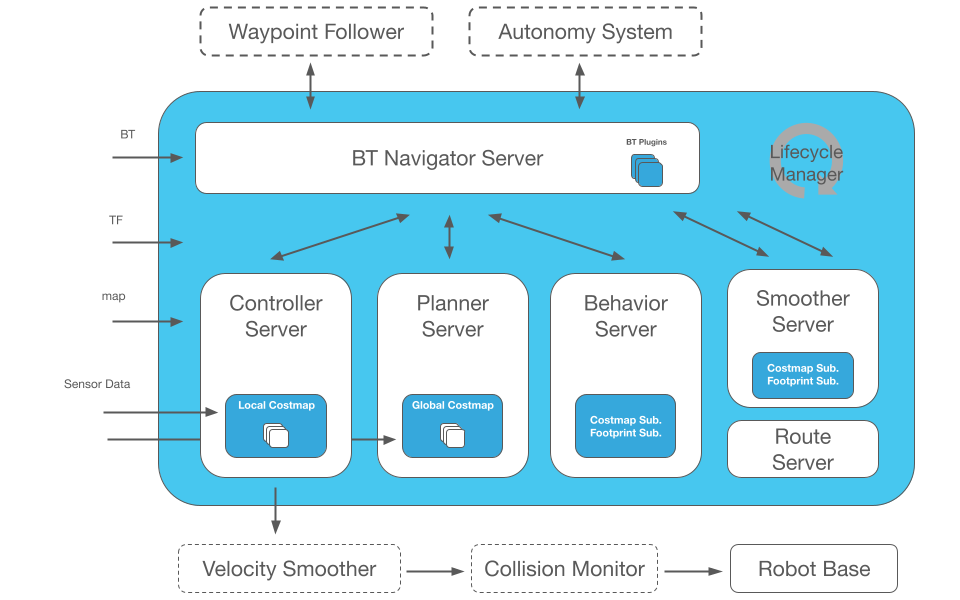
\includegraphics[width=14cm]{nav2_architecture}
}
\caption{Архитектура стэка Nav2}
\end{figure}

В Nav2 есть инструменты:
\begin{itemize}
	\item загрузки, обслуживания и хранения карт;
	\item локализации робота по предоставленной карте (SLAM предоставляет
		начальную карту);
	\item планирования полного пути через окружающую среду;
	\item управления роботом, чтобы он следовал по маршруту и динамически
		корректировался, чтобы избежать столкновений;
	\item сглаживания маршрутов, чтобы сделать их более непрерывными, плавными
		и/или выполнимыми.
	\item преобразование данных датчиков в модель окружающего мира;
	\item построение сложных и настраиваемых моделей поведения роботов с
		помощью деревьев поведения;
	\item выполнение заранее определенных действий в случае сбоя, вмешательства
		человека или других ситуаций;
	\item выполнение последовательных маршрутных точек, составляющих миссию;
	\item управление жизненным циклом программы и сторожевым таймером для
		серверов;
	\item простые динамически загружаемые модули для создания индивидуальных
		алгоритмов, поведений и т. д.
	\item мониторинг необработанных данных датчиков на предмет неминуемого
		столкновения или опасной ситуации;
\end{itemize}

\subsection{Анализ пакетов решающих задачу навигации, локализации и построения
карты}

Для навигации мобильной системы необходима карта, для построения которой
используют SLAM (Одновременную локализацию и построение карты). 

Алгоритмы SLAM можно разделить на две группы: более ранние алгоритмы,
использующие подходы, основанные на фильтрах Байеса , и более новые методы,
основанные на графах. Значимые реализации на основе фильтров, доступные в виде
пакетов \ros{}: GMapping и HectorSLAM. Cartographer и KartoSLAM являются
основными доступными реализациями на основе графов \cite{macenski2021slam}.

Рассмотрим пакеты ros{}, такие как: SLAM Toolbox и GMapping:
\begin{itemize}
	\item SLAM Toolbox -- использует подход оптимизации
		графов.
	\item GMapping \cite{grisetti2005improving} -- использует Rao–Blackwellized
		Particle Filter (Фильтр частиц с использование теоремы Рао — Блэквелла —
		Колмогорова )
\end{itemize}

В SLAM Toolbox есть возможность делать почти всё, что есть в любой другой
платной и бесплатной библиотеке SLAM. Это включает в себя:
\begin{itemize}
	\item обычный точечный 2D SLAM для мобильных роботов (карта,
		сохранение pgm-файла) с утилитами, такими как сохранение карт;
	\item продолжение уточнения, перестройки карты или продолжения построения
		карты сохраненного (сериализованного) графа позиций в любое время;
	\item пожизненное картирование: загрузите сохраненный граф позиций и
		продолжайте строить карту, одновременно удаляя лишнюю
		информацию из новых сканов;
	\item режим локализации на основе оптимизации, построенный на основе
		pose-графа. Возможность запуска режима локализации без предварительной
		карты для режима «лидарной одометрии» с локальным замыканием контуров;
	\item синхронный и асинхронный режимы отображения;
	\item объединение кинематических карт (в разработке находится техника
		объединения манипуляций с эластичным графом);
	\item оптимизационные решатели на основе плагинов с новым оптимизированным
		плагином на основе Google Ceres;
	\item плагин RVIZ для взаимодействия с инструментами;
	\item инструменты манипулирования графами в RVIZ для манипулирования узлами
		и связями во время отображения;
	\item сериализация карт и хранение данных без потерь.
\end{itemize}

В то время как пакет GMapping предлагает обёртку над алгоритмом,
описанным в статье \cite{grisetti2005improving}, не включая дополнительный
функционал который предоставляется SLAM Toolbox, предоставляя лишь возможность
настройки параметров алгоритма и получения построенной карты.

\begin{figure}[h]
\centering
	\fbox{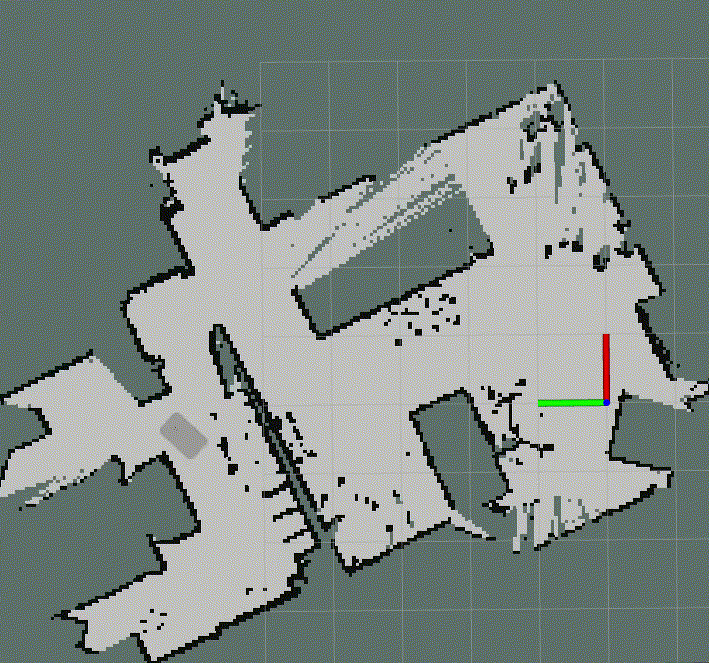
\includegraphics[width=7cm]{slam_toolbox_example}
\centering
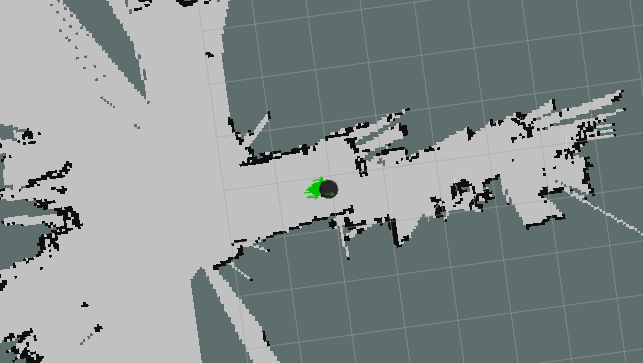
\includegraphics[width=7cm]{gmapping_example}
	}
	\caption{Пример построения карты используя SLAM Toolbox (слева) и GMapping
	(справа).}
\end{figure}

\subsection{Постановка целей и задач дипломного проектирования}
Фреймворки для разработки ПО для робототехники используют сервис для обмена
сообщения между модулями, но у этого архитектурного подхода есть ряд
недостатков: дополнительные затраты на сериализацию и десериализацию данных,
затраты на маршрутизацию сообщений, а также при использовании нескольких
программных модулей конечный программный продукт по своей сути является
распределённой системой, что вносит следующие недостатки:

\begin{itemize}
	\item проблемы с синхронизацией состояния, неконсистентность состояния;
	\item потеря сообщений;
	\item каскадный отказ системы;
	\item невозможность использования отладчика подключённого к одному
		исполняемому файлу для отладки всей системы навигации.
\end{itemize}

Исходя из этого, целью дипломного проектирования является разработка
программного средства осуществив вышеперечисленные оптимизации и устранив
вышеперечисленные недостатки, а также
реализовать необходимый набор функций, характерный для программных средств в
данной предметной области.

Для достижения поставленных целей следует решить следующие задачи: 
\begin{itemize}
	\item определить требования  к  разрабатываемому  программному  средству  и 
	составление спецификации, включающей их; 
	\item осуществить выбор  технологии  и  языка  программирования  для
		реализации программного средства; 
	\item провести проектирование архитектуры программного средства; 
	\item разработка алгоритмов для метода SLAM; 
	\item разработка алгоритмов для оценки местоположения; 
	\item разработка алгоритмов для поиска маршрута; 
	\item разработка алгоритмов для выполнения маршрута; 
	\item программирование и тестирование отдельных программных модулей; 
	\item тестирование готового программного средств.
\end{itemize}


\subsection{Алгоритмы фильтрации}

Оценка состояния динамических систем в условиях неопределённости является ключевой задачей в задачах навигации,
робототехники и обработки сигналов.
Существует большое количество алгоритмов, позволяющие решать задачу оценки состояния
c учётом заданных ограничений (например, ограничений по доступным вычислительным мощностям):
\begin{itemize}
	\item линейный фильтр Калмана (см. пункт $\ref{kf}$);
	\item расширенный фильтр Калмана (см. пункт $\ref{ekf}$);
	\item нелинейный фильтр Калмана (см. пункт $\ref{sec:ukf_info}$);
	\item фильтр частиц (см. пункт $\ref{particle_filter}$);
	\item комплиментарный фильтр;
	\item H$\infty$-фильтр.
\end{itemize}
Каждый метод анализируется с точки зрения его математической основы и применимости в задачах навигации.

\subsubsection{Фильтр Калмана}
\label{kf}
\hfill

Фильтр Калмана -- рекурсивный алгоритм,
обеспечивающий оптимальную оценку состояния линейной динамической системы с нормально распределёнными шумами.
Предположение, что шум системы нормально распределён является ключевым 
Динамику системы в момент времени \( k \) можно описывается уравнением момент времени:
\begin{align}
    \mathbf{x}_k &= \mathbf{F}_k \mathbf{x}_{k-1} + \mathbf{B}_k \mathbf{u}_k + \mathbf{w}_k, \label{eq:kalman_state} \\
    \mathbf{z}_k &= \mathbf{H}_k \mathbf{x}_k + \mathbf{v}_k. \label{eq:kalman_meas}
\end{align}

где \(\mathbf{x}_k\) -- вектор переменных состояния, \(\mathbf{z}_k\) -- вектор переменных измерений,
\(\mathbf{u}_k\) -- управляющие переменные, \(\mathbf{w}_k\) шум процесса,
\(\mathbf{v}_k \) -- шум измерений, \(\mathbf{F}_k\) -- матрица перехода состояния,
\(\mathbf{B}_k\) -- матрица управления, \(\mathbf{H}_k\) -- матрица измерений.

Переменные состояния (\(\mathbf{x}_k\)) описывают характеристики системы на временном шаге \( k \).
Переменные состояния полностью определяют её динамическое поведение.
Переменные измерения (\(\mathbf{z}_k\)) представляют наблюдаемые данные, получаемые от датчиков на шаге \( k \). 
Они описываются моделью измерений (см. уравнение \ref{eq:kalman_meas})
Управляющие переменные (\(\mathbf{u}_k\)) описывают внешние воздействия на систему, влияющие на её динамику.
Они входят в уравнение состояния и считаются известными, предоставляемыми системой управления.
Например, команды управления для перемещающегося средства.

Матрица перехода состояния \(\mathbf{F}_k\) описывает эволюцию состояния системы \(\mathbf{x}_k\) во времени без учёта управления и шума.
Матрица управления \(\mathbf{B}_k\) описывает влияние управляющего сигнала \(\mathbf{u}_k\) на состояние системы. Она также входит в уравнение состояния и имеет размер \(n \times m\), где \(m\) --- размерность \(\mathbf{u}_k\).

В идеальных условиях, шум процесса \(\mathbf{w}_k\) и шум измерений \(\mathbf{м}_k\)
полагаются равны 0. Пользователь может самостоятельно изменять 
значения шума в зависимости от степени доверия системе или измерениям.


Все переменные, в зависимости от возможности произвести наблюдение за значением,
можно разделить на скрытые и явные зависимости.
К скрытым переменным относят:
\begin{itemize}
    \item переменные состояния $\mathbf{x}_k$; 
    \item шум процесса $\mathbf{w}_k$.
\end{itemize}

К явным переменным относят:
\begin{itemize}
    \item переменные измерений $\mathbf{z}_k$; 
    \item управляющие переменные $\mathbf{u}_k$; 
    \item шум измерений $\mathbf{v}_k$.
\end{itemize}

Работа фильтра Калмана основана на последовательном выполнении этапов предсказания (predict) и 
коррекции (update).

На этапе предсказания выполняется расчёт 
априорной оценки переменных состояния (см. уравнение \ref{x_predict})
и априорной оценки ковариация ошибка системы (см. уравнение \ref{p_predict}).
\begin{align}
\hat{\mathbf{x}}_{k|k-1} &= \mathbf{F}_k \hat{\mathbf{x}}_{k-1|k-1} + \mathbf{B}_k \mathbf{u}_k, \label{x_predict}\\
\mathbf{P}_{k|k-1} &= \mathbf{F}_k \mathbf{P}_{k-1|k-1} \mathbf{F}_k^T + \mathbf{Q}_k. \label{p_predict}.
\end{align}

Этап коррекции обновляет априорную оценку с учётом измерений, полученных с использованием датчиков.
Для этого вычисляются коэффициент усиления Калмана \(\mathbf(K)_k\) (см. уравнение \ref{kf_gain}),
апостериорная оценка состояния \(\mathbf{x}_{k|k}\) (см. уравнение \ref{x_update}),
и апостериорная ковариация ошибки \(\mathbf{P}_{k|k}\) (см. уравнение \ref{p_update}).

\begin{equation}
\label{kf_gain}
\mathbf{K}_k = \mathbf{P}_{k|k-1} \mathbf{H}_k^T (\mathbf{H}_k \mathbf{P}_{k|k-1} \mathbf{H}_k^T + \mathbf{R}_k)^{-1},
\end{equation}

\begin{equation}
\label{x_update}
\hat{\mathbf{x}}_{k|k} = \hat{\mathbf{x}}_{k|k-1} + \mathbf{K}_k (\mathbf{z}_k - \mathbf{H}_k \hat{\mathbf{x}}_{k|k-1}),
\end{equation}

\begin{equation}
\label{p_update}
\mathbf{P}_{k|k} = (\mathbf{E} - \mathbf{K}_k \mathbf{H}_k) \mathbf{P}_{k|k-1}.
\end{equation}
\\

Коэффициент \(\mathbf{K}_k\) балансирует доверие к модели и измерениям, снижая неопределённость.

\subsubsection{Расширенный фильтр Калмана (Extended Kalman Filter)}
\label{ekf}
\hfill


Расширенный фильтр Калмана (EKF) адаптирует фильтр Калмана (KF) для нелинейных систем:

\begin{align}
    \mathbf{x}_k &= \mathbf{f}(\mathbf{x}_{k-1}, \mathbf{u}_k) + \mathbf{w}_k, \\
    \mathbf{z}_k &= \mathbf{h}(\mathbf{x}_k) + \mathbf{v}_k.
\end{align}

Линеаризация выполняется с помощью матриц Якоби \(\mathbf{F}_k = \frac{\partial \mathbf{f}}{\partial \mathbf{x}}\big|_{\hat{\mathbf{x}}_{k-1|k-1}}\) и \(\mathbf{H}_k = \frac{\partial \mathbf{h}}{\partial \mathbf{x}}\big|_{\hat{\mathbf{x}}_{k|k-1}}\). Этапы предсказания и коррекции аналогичны фильтру Калмана, но ошибки линеаризации снижают точность при сильной нелинейности.

\subsubsection{Нелинейный фильтр Калмана (Unscented Kalman Filter)}
\label{sec:ukf_info}
\hfill

UKF использует сигма-точки для обработки нелинейностей без линеаризации. Сигма-точки генерируются на основе \(\hat{\mathbf{x}}_{k-1|k-1}\) и \(\mathbf{P}_{k-1|k-1}\), затем распространяются через \(\mathbf{f}\) и \(\mathbf{h}\):
\begin{align}
    \hat{\mathbf{x}}_{k|k-1} &= \sum w_i \mathbf{f}(\mathbf{x}_i), \\
    \mathbf{P}_{k|k-1} &= \sum w_i (\mathbf{f}(\mathbf{x}_i) - \hat{\mathbf{x}}_{k|k-1})(\mathbf{f}(\mathbf{x}_i) - \hat{\mathbf{x}}_{k|k-1})^T + \mathbf{Q}_k.
\end{align}
Для состояния \(\mathbf{x}_{k-1|k-1}\) с оценкой 
\(\hat{\mathbf{x}}_{k-1|k-1}\) и ковариацией \(\mathbf{P}_{k-1|k-1}\) 
генерируется \(2n + 1\) сигма-точек, где \(n\)  -- это размерность вектора состояний \(\mathbf{x}_k\).
Для генерации точек используется следующий алгоритм:

\begin{enumerate}
    \item Вычисление масштабирующего параметра:
    \[
    \lambda = \alpha^2 (n + \kappa) - n,
    \]
    где \(\alpha\) (\(10^{-3} \leq \alpha \leq 1\)) контролирует разброс, \(\kappa\) (обычно \(3 - n\)) --- параметр настройки.
    \item Генерация сигма-точек:
    \[
    \mathbf{x}_{k-1}^{(0)} = \hat{\mathbf{x}}_{k-1|k-1},
    \]
    \[
    \mathbf{x}_{k-1}^{(i)} = \hat{\mathbf{x}}_{k-1|k-1} + (\sqrt{(n + \lambda) \mathbf{P}_{k-1|k-1}})_i, \quad i = 1, \dots, n,
    \]
    \[
    \mathbf{x}_{k-1}^{(i)} = \hat{\mathbf{x}}_{k-1|k-1} - (\sqrt{(n + \lambda) \mathbf{P}_{k-1|k-1}})_{i-n}, \quad i = n+1, \dots, 2n,
    \]
    где \((\sqrt{(n + \lambda) \mathbf{P}_{k-1|k-1}})_i\) --- \(i\)-й столбец разложения Холецкого.
    \item Назначение весов:
    \[
    w_m^{(0)} = \frac{\lambda}{n + \lambda}, \quad w_m^{(i)} = \frac{1}{2(n + \lambda)}, \quad i = 1, \dots, 2n,
    \]
    \[
    w_c^{(0)} = \frac{\lambda}{n + \lambda} + (1 - \alpha^2 + \beta), \quad w_c^{(i)} = \frac{1}{2(n + \lambda)}, \quad i = 1, \dots, 2n,
    \]
    где \(\beta \approx 2\) для нормального распределения.
\end{enumerate}

В общем случае, UKF работает более точно, чем EKF:
\begin{itemize}
    \item высокая точность при сильной нелинейности, так как сигма-точки лучше аппроксимируют распределение;
    \item отсутствие необходимости вычислять производные, что упрощает реализацию для сложных функций.
\end{itemize}

\subsubsection{Фильтр частиц (Particle Filter)}
\label{particle_filter}
\hfill

Фильтр частиц (PF) представляет распределение состояния множеством частиц \(\{\mathbf{x}_k^{(i)}, w_k^{(i)}\}\). 
Этот метод оценки состояния динамической системы, основанный на методе Монте-Карло.
PF особенно эффективен для нелинейных систем с шумами, которые распределены не нормально.
То есть в тех системах, где фильтр Калмана и его модификации (EKF, UKF) могут быть недостаточно точны.

Система описывается уравнениями:
\begin{align}
    \mathbf{x}_k &= \mathbf{f}(\mathbf{x}_{k-1}, \mathbf{u}_k, \mathbf{w}_k), \label{eq:pf_state} \\
    \mathbf{z}_k &= \mathbf{h}(\mathbf{x}_k, \mathbf{v}_k), \label{eq:pf_meas}
\end{align}

где \(\mathbf{x}_k\) -- переменные состояния, \(\mathbf{u}_k\) -- управляющие переменные,
\(\mathbf{z}_k\) -- измерения,
\(\mathbf{w}_k\) -- шум процесса,
\(\mathbf{v}_k\) — шум измерения,
\(\mathbf{f}\), \(\mathbf{h}\) — нелинейные функции. 

Апостериорное распределение аппроксимируется:
\begin{equation}
    p(\mathbf{x}_k | \mathbf{z}_{1:k}) \approx \sum_{i=1}^N w_k^{(i)} \delta(\mathbf{x}_k - \mathbf{x}_k^{(i)}),
\end{equation}
где \(\delta\) — дельта-функция Дирака, \(\sum_{i=1}^N w_k^{(i)} = 1\).


Работа PF состоит из трёх этапов: предсказание, обновление весов и пересборку (ресэмплинг).

На этапе предсказания каждая частица обновляется по модели системы (см. уравнение \ref{pf_predict}).
Все частицы формируют априорное распределение \(\{\mathbf{x}_k^{(i)}\}_{i=1}^N\).

\begin{equation}
	\mathbf{x}_k^{(i)} = \mathbf{f}(\mathbf{x}_{k-1}^{(i)}, \mathbf{u}_k, \mathbf{w}_k^{(i)}), \quad \mathbf{w}_k^{(i)} \sim p(\mathbf{w}_k). \label{pf_predict}
\end{equation}


На этапе обновления весов веса частиц обновляются по принципу правдоподобия:

\begin{equation}
	w_k^{(i)} \propto w_{k-1}^{(i)} p(\mathbf{z}_k | \mathbf{x}_k^{(i)}).
\end{equation}

где для нормально распределённого шума \(\mathbf{v}_k \sim \mathcal{N}(0, \mathbf{R}_k)\):

\begin{align}
    p(\mathbf{z}_k | \mathbf{x}_k^{(i)}) = \frac{1}{\sqrt{(2\pi)^p |\mathbf{R}_k|}} \exp\left(-\frac{1}{2} (\mathbf{z}_k - \mathbf{h}(\mathbf{x}_k^{(i)}))^T \mathbf{R}_k^{-1} (\mathbf{z}_k - \mathbf{h}(\mathbf{x}_k^{(i)}))\right).
\end{align}

После веса всех частиц нормируются:

\begin{equation}
    w_k^{(i)} = \frac{w_k^{(i)}}{\sum_{j=1}^N w_k^{(j)}}.
\end{equation}

На этапе ресэмплинга устраняется вырождение частиц
и осуществляется выбор нового набора частиц \(\{\mathbf{x}_k^{(i)}\}_{i=1}^N\) с вероятностями,
пропорциональными \(w_k^{(i)}\). После ресэмплинга \(w_k^{(i)} = 1/N\) состояние системы 
определяется как:

\begin{equation}
    \hat{\mathbf{x}}_k = \sum_{i=1}^N w_k^{(i)} \mathbf{x}_k^{(i)}.
\end{equation}

\subsection{AHRS}
\label{subsec:ahrs}

Система ориентации и курса (Attitude and Heading Reference System или AHRS) предназначена для оценки
ориентации объекта: углов крена (roll), тангажа (pitch) и рысканья (yaw).
В задачах навигации, подобных тем, где применяются фильтр частиц (PF) или фильтры Калмана,
AHRS играет ключевую роль в определении ориентации.
Основные источники данных, для которых используется AHRS: 
\begin{itemize}
    \item гироскопы (\(\boldsymbol{\omega} = [\omega_x, \omega_y, \omega_z]^T\)) для измерения угловой скорости.
    \item акселерометры (\(\mathbf{a} = [a_x, a_y, a_z]^T\)) для оценки крена и тангажа через вектор силы тяжести.
    \item магнитометры (\(\mathbf{m} = [m_x, m_y, m_z]^T\)) для определения рысканья относительно магнитного севера.
\end{itemize}

Ориентация представляется в системе кватернионом \(\mathbf{q} = [q_0, q_1, q_2, q_3]^T\), что позволяет
избежать блокировки кардана (gimbal lock).

Применение AHRS ограничивается рядом внешних условий:

\begin{enumerate}[label=\arabic*]
    \item Наличие магнитных помех искажают показания магнитометров.
    \item Дрейф гироскопов требует внешней коррекции. Использование алгоритмов фильтрации
	    с AHRS позволяет произвести корректировку дрейфа гироскопов.
    \item AHRS не моделирует положение и линейную скорость.
\end{enumerate}

\subsection{Оценка измерений в AHRS}

Для оценки ориентации в AHRS принято использовать один из двух алгоритмов: фильтр Маджвика или фильтр Махони.

\subsubsection{Фильтр Маджвика}
\hfill

Фильтр Маджвика использует градиентный спуск для минимизации ошибки гироскопа 
с коррекцией от акселерометра и магнитометра. Он оценивает кватернион ориентации
\(\mathbf{q}_t\) путём численного интегрирования:

\begin{equation}
    \dot{\mathbf{q}}_t = \dot{\mathbf{q}}_{\omega, t} - \beta \dot{\mathbf{q}}_{\epsilon, t},
\end{equation}
где
    \(\dot{\mathbf{q}}_{\omega, t} = \frac{1}{2} \mathbf{q}_{t-1} \otimes \begin{bmatrix} 0 \\ 
    \boldsymbol{\omega}_t \end{bmatrix}\) -- изменения ориентации от гироскопа \(\boldsymbol{\omega}_t\);
    \(\dot{\mathbf{q}}_{\epsilon, t}\) -- 
    численное значение ошибки, вычисленное градиентным спуском из данных акселерометра 
    (\(\mathbf{a}_t\)) и магнитометра (\(\mathbf{m}_t\));
    \(\beta\) -- коэффициент доверия к фильтру ($\beta \in [0.1, 1]$).

Основными преимуществами фильтра Маджвика являются:
\begin{itemize}
	\item высокая точность вычисления ориентации;
	\item эффективная компенсация дрейфа гироскопа.
\end{itemize}

\subsubsection{Фильтр Махони}
\hfill

Фильтр Махони основан на нелинейном комплементарном фильтре на группе \(SO(3)\).
Он минимизирует ошибку между измеренными и эталонными векторами с помощью пропорционально-интегрального (PI)
компенсатора. Ориентация обновляется как:

\begin{equation}
    \dot{\mathbf{q}}_t = \frac{1}{2} \mathbf{q}_t \otimes \begin{bmatrix} 0 \\ \boldsymbol{\omega}_t + \mathbf{e}_t \end{bmatrix},
\end{equation}
где
    \(\mathbf{e}_t = k_P \boldsymbol{\omega}_{\text{err}} + k_I \int \boldsymbol{\omega}_{\text{err}} \, dt\) --
    коррекция, основанная на ошибке \(\boldsymbol{\omega}_{\text{err}}\), 
    вычисленной как векторное произведение измеренных и предсказанных векторов.
    \(k_P \approx 1\), \(k_I \approx 0.3\) -- PI-компенсатора.

К основным преимуществам фильтра Махони относят:
\begin{itemize}
	\item быстрая сходимость;
	\item низкая вычислительная сложность;
\end{itemize}

Фильтр требует тщательного выбора параметров \(k_P\), \(k_I\). По сравнению с фильтром Маджвика, 
фильтр Махони хуже оценивает ориентацию в пространстве.


Таким образом, оба фильтра имеют место быть для различных условий применения.
Фильтр Маджвика предоставляет большую точность на низкой частоте отправке данных.
Фильтр Махони используются на системах с ограниченной вычислительной мощностью.

\subsection{Глобальные планировщики}
Глобальные планировщики предназначены для построения маршрута от начальной точки до цели
в известной или частично известной среде, обычно представленной в виде графа или сетки.
В качестве глобальных планировщиков используют:
\begin{itemize}
	\item алгоритм Дейкстры;
	\item алгоритм A*;
	\item алгоритм RRT.
\end{itemize}

\subsubsection{Алгоритм Дейкстры}
\hfill

Алгоритм Дейкстры служит для поиска кратчайшего пути в графе с неотрицательными весами рёбер.
Начиная с начальной вершины, алгоритм последовательно обновляет расстояния до всех остальных вершин,
выбирая на каждом шаге вершину с минимальным текущим расстоянием.
Для выбранной вершины проверяются её соседи, и расстояния до них обновляются,
если найден более короткий путь.
Процесс продолжается до обработки всех вершин или достижения цели.

Математически алгоритм минимизирует расстояние до вершины $v$ по формуле:
\begin{equation}
d[v] = \min_{u \in V} \{ d[u] + w(u, v) \},
\end{equation}
где $d[v]$ -- кратчайшее расстояние от начальной вершины до $v$,
а $w(u, v)$ -- вес ребра между вершинами $u$ и $v$.

Алгоритм гарантирует оптимальность пути,
но для больших графов требует значительных вычислений,
с временной сложностью $O((V + E) \log V)$ при использовании кучи.

\subsubsection{Алгоритм A*}
\hfill

Алгоритм A* улучшает подход Дейкстры,
добавляя эвристическую функцию для ускорения поиска.
Каждая вершина оценивается по сумме стоимости пути от начальной точки ($g(v)$)
и эвристической оценки расстояния до цели ($h(v)$).
Выбирается вершина с минимальной суммой $f(v) = g(v) + h(v)$.
Эвристика должна быть допустимой, то есть не переоценивать истинное расстояние: $h(v) \leq h^*(v)$,
где $h^*(v)$ -- реальное расстояние до цели.

Логику алгоритма можно описать формулой:
\begin{equation}
f(v) = g(v) + h(v).
\end{equation}

A* эффективен для планирования в сетках или графах,
особенно при использовании точной эвристики для сокращения количество проверяемых вершин.

\subsubsection{RRT (Rapidly-exploring Random Tree)}
RRT -- алгоритм для планирования маршрутов в непрерывных высокомерных пространствах. 
Алгоритм строит дерево, начиная с начальной конфигурации, 
путём случайной выборки точек в конфигурационном пространстве.
Для каждой случайной точки находится ближайший узел дерева,
и к нему добавляется новая конфигурация на расстоянии $\delta$ в направлении случайной точки,
если она свободна от препятствий. Процесс повторяется до достижения цели или превышения лимита итераций.

Упрощённо работу алгоритма можно описать формулой:
\begin{equation}
q_{\text{new}} = q_{\text{near}} + \delta \cdot \frac{q_{\text{rand}} - q_{\text{near}}}{\| q_{\text{rand}} - q_{\text{near}} \|}.
\end{equation}

RRT вероятностно полный, но не обеспечивает оптимальность пути.

\subsection{Локальные планировщики}
Локальные планировщики корректируют движение робота в реальном времени, учитывая динамику и локальные препятствия.

\subsubsection{DWA (Dynamic Window Approach)}
DWA предназначен для выбора оптимальной пары скоростей (линейной и угловой) с учётом кинематических
ограничений движущегося объекта. Алгоритм формирует  множество допустимых скоростей (динамическое окно),
ограниченных текущим состоянием и ускорениями:

\begin{equation}
W_d = \{ (v, \omega) \mid v \in [v_{\min}, v_{\max}],	\omega \in [\omega_{\min}, \omega_{\max}] \}.
\end{equation}

Для каждой пары скоростей моделируется траектория,
оцениваемая по ориентации к цели, расстоянию до препятствий и величине скорости.
Выбирается пара скоростей, минимизурующая целевую функцию $G(v, \omega)$:

\begin{equation}
(v^*, \omega^*) = \min_{(v, \omega) \in W_d} G(v, \omega),
\end{equation}

DWA активно используются для дифференциальных роботов. Но основным недостатком алгоритма
является проблема застревания в локальных минимумах целевой функции.

\subsubsection{TEB (Timed Elastic Band)}
\hfill

TEB оптимизирует траекторию, представляя её как эластичную ленту,
которая деформируется для минимизации энергетический потерь на перемещение.
Траектория состоит из набора конфигураций (состояний) $\{q_1, q_2, \dots, q_n\}$, 
соединённых временными интервалами $\Delta T_i$. 

Алгоритм TEB оптимизирует эти конфигурации и интервалы, минимизируя целевую функцию:
\begin{equation}
	J(B) = \sum_{i=1}^{n-1} \left( w_1 \| q_{i+1} - q_i \|^2 + w_2 \Delta T_i^2 + w_3 \sum_{\text{obj}} \text{obj}(q_i, \text{p})^{-2} \right),
\end{equation}
где первый член обеспечивает компактность траектории, 
второй -- минимизацию времени, 
а третий -- избегание препятствий.

Конфигурации учитывают кинематические ограничения, такие как максимальная скорость:

\begin{equation}
v_i = \frac{q_{i+1} - q_i}{\Delta T_i}, \quad \| v_i \| \leq v_{\max}.
\end{equation}

По сравнению с DWA, TEB требует большей вычислительной сложностью,
но позволяет описать модель перемещения более точно. 
